\documentclass{article}

\usepackage{graphicx}

\usepackage{listings}
\usepackage{xcolor}

\usepackage{hyperref}

\lstdefinelanguage{Cypher}{
  keywords={MATCH, RETURN, WHERE, CREATE, DELETE, SET, WITH, MERGE},
  sensitive=true,
  morecomment=[l]{//},
  morestring=[b]"
}

\lstset{
  language=Cypher,
  basicstyle=\ttfamily\small,
  keywordstyle=\color{blue}\bfseries,
  stringstyle=\color{red},
  commentstyle=\color{green!50!black},
  numbers=left,
  numberstyle=\tiny\color{gray},
  stepnumber=1,
  numbersep=5pt,
  showstringspaces=false,
  breaklines=true,
  frame=single
}


\title{Basket}
\author{
    MATTHEWS Louis-Marie,
    OUNES Sarah
}

\begin{document}

\maketitle

\tableofcontents

\section{Exploring and preparing the dataset}

\subsection{Basic EDA}

The dataset we are using is the \verb|Basketball_women.json| dataset. As for any data science project,  we begin with an EDA\footnote{Exploratory Data Analysis.}

For this, we use Python with the Pandas library, as well as a notebook as it makes prototyping and seeing the result very fast and convenient. We use these tools to get an idea of the structure and the volume of the data.

\begin{figure}[ht]
    \centering
    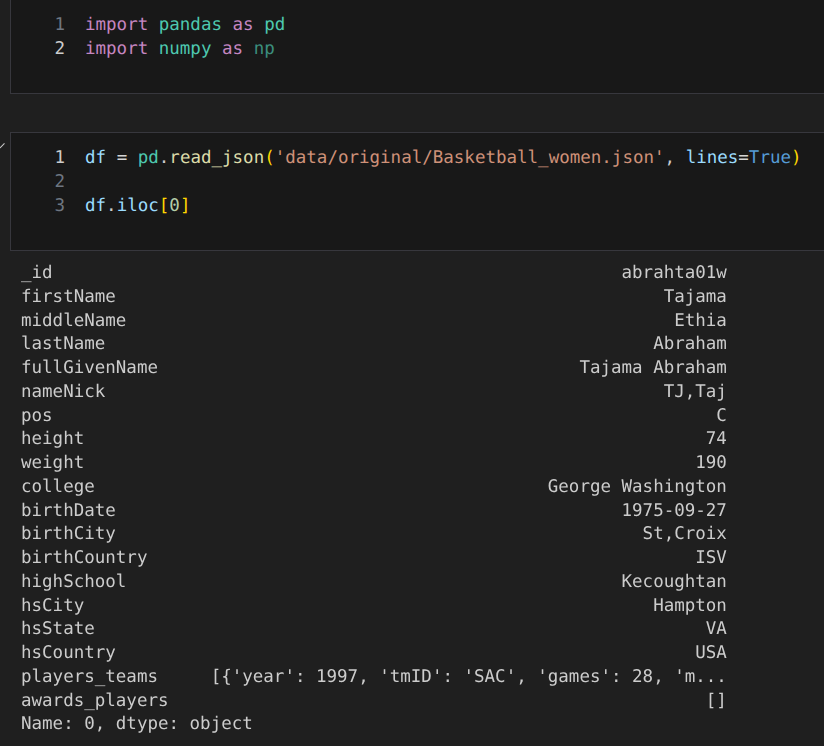
\includegraphics[width=\linewidth]{image.png}
    \caption{We use Pandas for very basic EDA.}
    \label{fig:eda}
\end{figure}

By looking at the first row, as well as at the result of \verb|df.info()| and the non-empty values for the columns \verb|players_teams| and \verb|awards_players|, we can identify several distinct entities that will our constitute the types of the future nodes of our graph. Those are:

\begin{itemize}
    \item Player,
    \item Award,
    \item College,
    \item High-School,
    \item and Team.
\end{itemize}

Player is the only node with a one-way relationship towards all other node types. In certain cases, as for its relationship with \texttt{Team}, the relationship has parameters (e.g. the year, the number of goals, etc).

\subsection{Preparing the data}

We split the dataset into 5 smaller CSV files. CSV files are easier to import into Neo4j Desktop. Each dataset corresponds to a node type. The Player node type is the only one with properties, all the others only contain an identifier for the specific node. This means we do not need to create datasets for relationships with the Player node type, we can simply package them with the node type.

Those datasets are:

\begin{itemize}
    \item \verb|awards.csv|: A list of awards, and the relationships between players and awards, as well as relationship information (when was the award won by the player, etc).
    \item \verb|colleges.csv|
    \item \verb|high_schools.csv|
    \item \verb|players_teams.csv|: Similar to \verb|awards.csv|, but for teams.
    \item \verb|players.csv|: Lists players information, and their high school and college they attended.
\end{itemize}

\section{Importing the data into Neo4j Desktop}

Neo4j Desktop makes it convenient and easy to import data. From its graphical user interface, and after creating an instance and a database for our project, it sufficed to import the CSV files, and determine the different node labels (the name of the type), properties, as well as the relationships.

\begin{figure}[htbp]
    \centering
    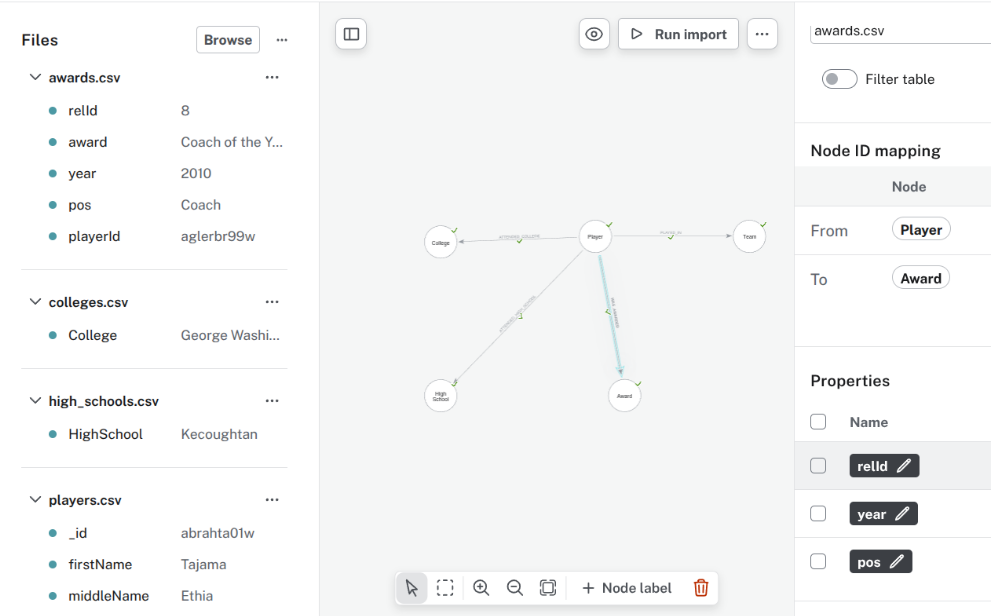
\includegraphics[width=\linewidth]{import.png}
    \caption{Importing data into Neo4j is intuitive.}
    \label{fig:import}
\end{figure}

\begin{figure}[htbp]
    \centering
    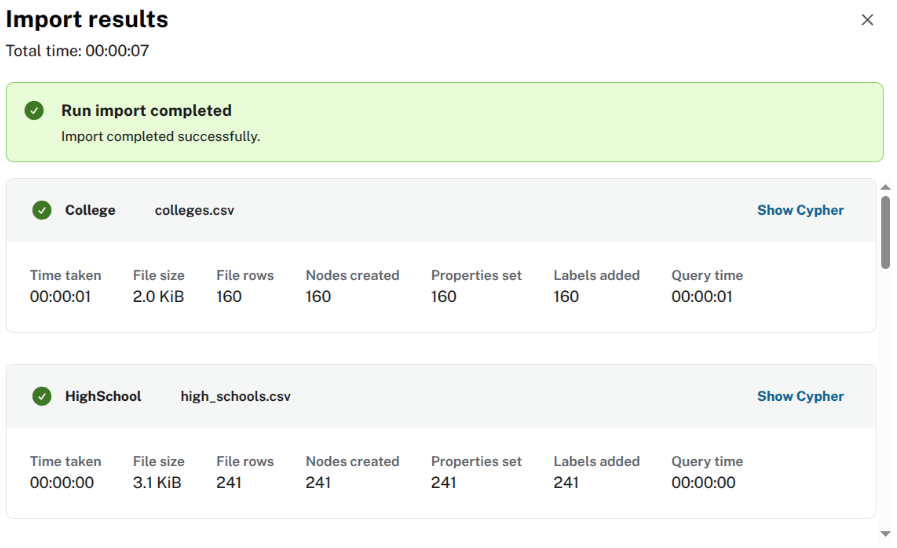
\includegraphics[width=\linewidth]{import_success.png}
    \caption{Importing data is successful.}
    \label{fig:import_success}
\end{figure}

\section{Exploring the data with Neo4j}

With 1878 nodes and relationships, the dataset is huge, and not everything can be seen from the Explore section of Neo4j Desktop. (Fig. \ref{fig:huge})

\begin{figure}[htbp]
    \centering
    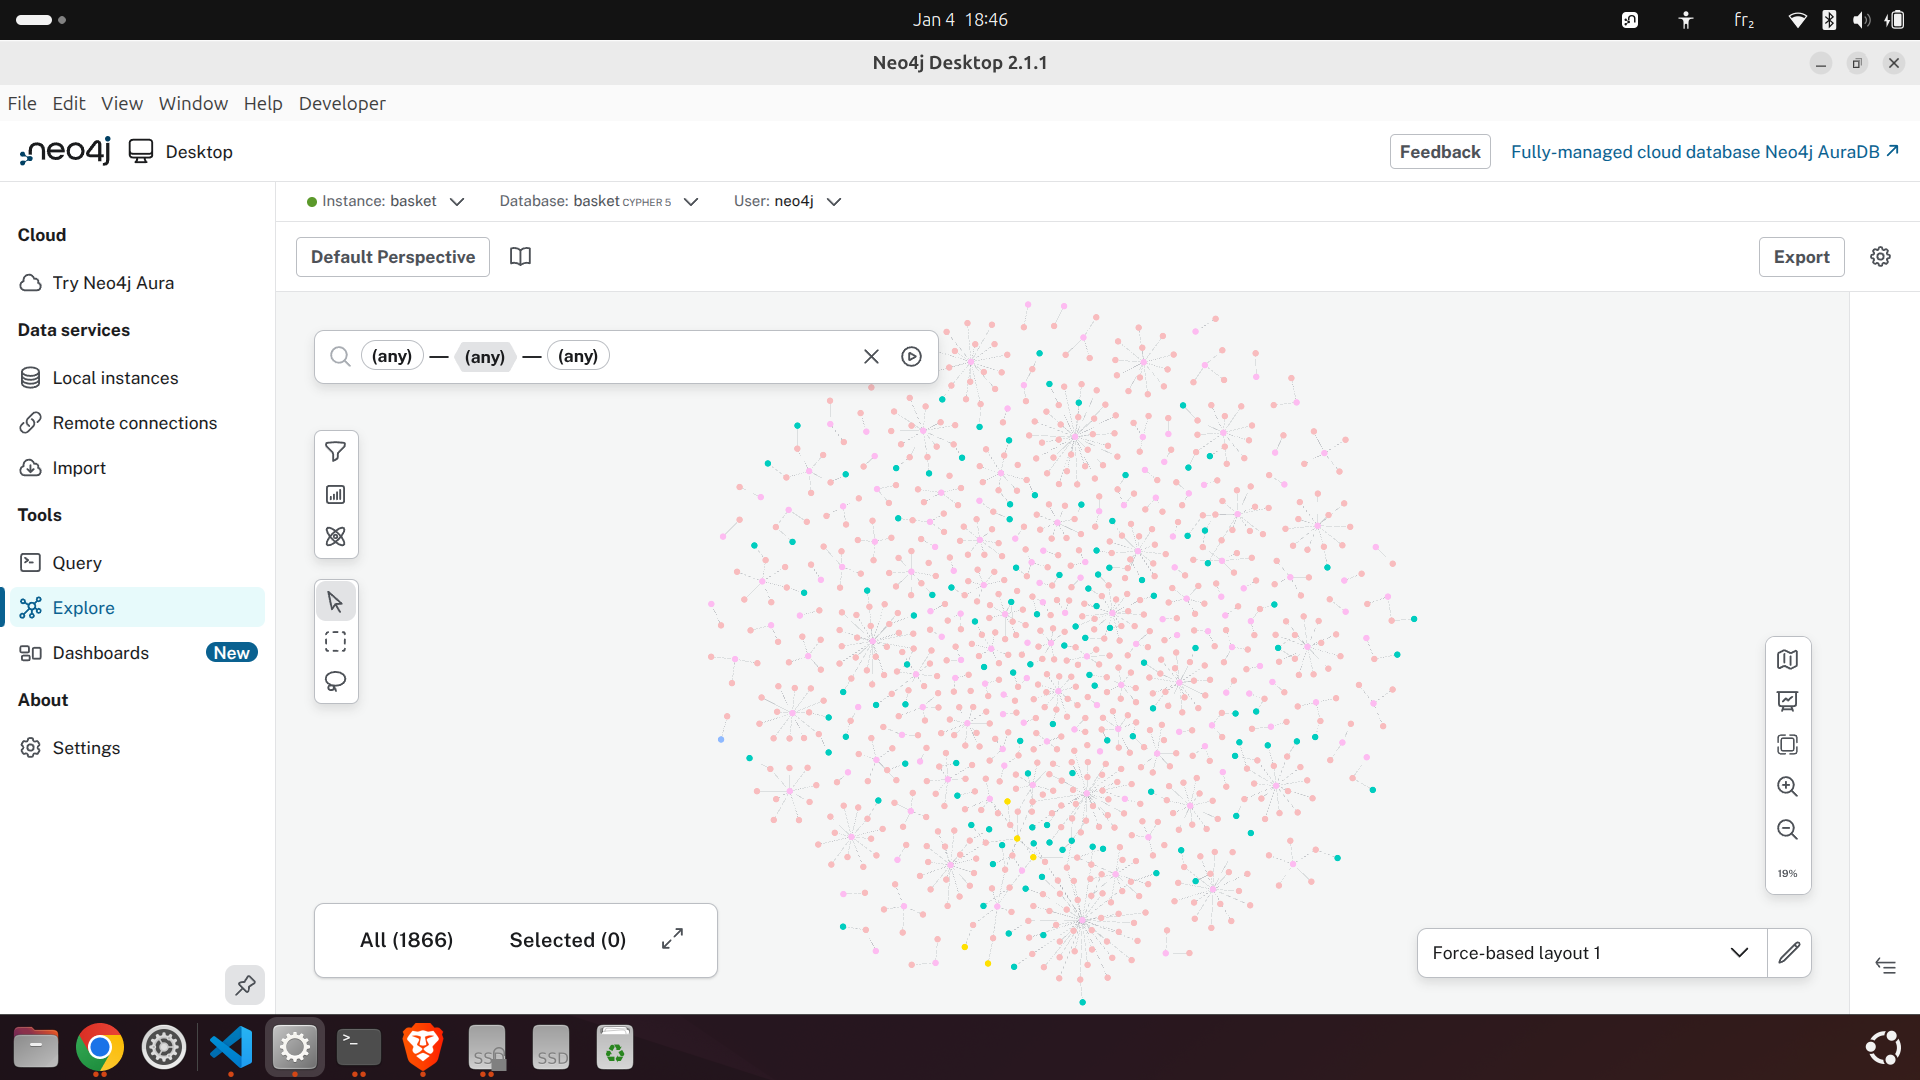
\includegraphics[width=\linewidth]{lot_data.png}
    \caption{The dataset is huge and not everything can be shown at the same time.}
    \label{fig:huge}
\end{figure}

\subsection{Creating a projection}

First, we must understand what a \textbf{projection} is. This is a very important concept. It can be useful to compare them to \textbf{Views} in traditionnal RDBMS. They are \textit{in-memory} graphs, made from a subset of nodes and relationships of the database graph, and sometimes transformed. As they exist in the DBMS' memory only, they are erased when the instance shuts down. This means they are not part of the database's files.

Projections are not meant to be used like views however. They are not intented to be displayed in Neo4j Desktop's Explorer for instance. They are intended to facilitate the running of algorithms on our data. Indeed, because they are in-memory and not on disk, algorithms can run faster. In addition, projections are decoupled from the database, which prevents accidental modification and makes it possible to create projections with certain caracterisics, i.e. only considering players from a certain school for instance.

Now that we understand what a projection is and what purpose they serve, let's create one in Neo4j.

\begin{figure}[htbp]
    \centering
    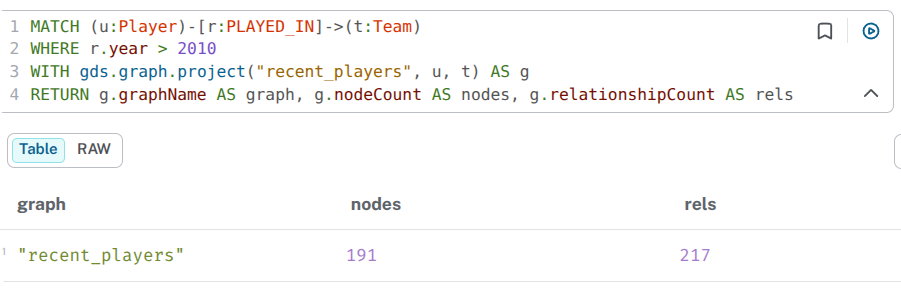
\includegraphics[width=\linewidth]{creating_proj.png}
    \caption{Creating a projection named recent\_players}
    \label{fig:creating_proj}
\end{figure}

Here, we create a projection based on the result of a \textbf{Cypher\footnote{Neo4j's DSL} query}. This is done by passing the output of the query, which always consists of a table of rows even when shown as a graph, to a \textbf{Procedure} from the \textbf{GDS plugin}. The GDS plugin then creates a projection (hence, "project") from the query's result.

We introduced three important terms: \textbf{Procedure}, \textbf{Plugin}, and \textbf{GDS}.

\begin{itemize}
    \item A \textbf{Procedure} is a function that can modify the database or run advanced algorithms. They are not part of the Cyper DSL. Instead, they are provided by plugins and can be called from within a Cypher query. (More on that later.)
    \item A \textbf{Plugin} extends the functionalities of Neo4j. Its installation is tied to a specific instance, i.e. a Neo4j server, and not to a database or to a Neo4j Desktop installation.
    \item \textbf{GDS} is an official plugin that provides advanced algorithms for analysing graphs.
\end{itemize}

In the following code snippet, we create a projection of the players with a team and who were awarded at least one award:

\begin{lstlisting}
    MATCH (u:Player)-[r:PLAYED_IN]->(t:Team)
    WHERE (u)-[:WAS_AWARDED]->(:Award)
    WITH gds.graph.project("recent_players", u, t) AS g
    RETURN g.graphName AS graph, g.nodeCount AS nodes, g.relationshipCount AS rels
\end{lstlisting}

There are simpler and more useful manners to create projections, for instance:

\begin{lstlisting}
CALL gds.graph.project("player_teams", ["Player", "Team"], "*", {PLAYED_IN: {orientation: 'UNDIRECTED'}})
\end{lstlisting}
 
We have \verb|undirectedRelationshipTypes| to make relationships undirected. Certain algorithms and metrics, such as the calculation of node degrees, only consider certain edge orientations. In addition, because there is only one edge type which only indicates a relationship between two different node types, there is no orientation.

This creates a projection with all players and all their relationships with teams. This effectively turns our $k$-partite graph into a bipartite one. But, gee, what is a bipartite graph?

\subsubsection{Creating a bipartite graph}

The graph we created by importing the CSVs that were transformed using Pandas is a \textbf{$k$-partite graph}. This is because we have several types of nodes and edges only between types. Certain algorithms only run on monopartite or bipartite graphs however, meaning graphs with one node type and relationship type in the former case and two partitions and with edges only between those partitions in the latter case. \footnote{"Most graph algorithms are designed to be executed on a monopartite network, where only a single node and relationship type are present." \url{https://www.oreilly.com/library/view/graph-algorithms-for/9781617299469/OEBPS/Text/ch06.htm}}

In general, as we lower the $k$ of our $k$-partite graph, we lose information gradually. For this reason, we will first make a bipartite projection from our graph, then a monopartite one.

We create the bipartite graph by only condidering the "Player" and the "Team" nodes, as they are the relationships with the most information. High school and college are already stored as properties of the "Player" node. \footnote{We could decide to create relationships between players who share the same high school and college, but not only do we not lose information yet (these informations are still stored in the node's properties), this could also result in the creation of artificial edges and huge, misleading cliques.}

So, creating our bipartite graph is just a matter of only creating the "Player" and "Team" nodes. We do this by calling the \verb|gds.graph.project()| \textbf{procedure} of the GDS \textbf{plugin}, which results in a new \textbf{projection}\footnote{Oh yeah, the GDS Plugin's Procedure to create a Projection! You Sir, are a mouthful!}. (Fig. \ref{fig:creating_bipartite})



\begin{figure}[htbp]
    \centering
    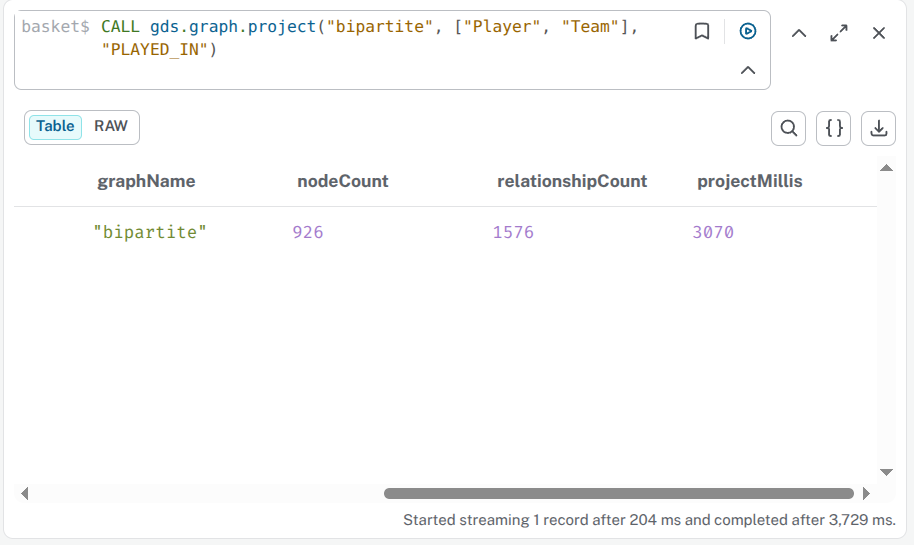
\includegraphics[width=\linewidth]{creating_bipartite.png}
    \caption{Creating a bipartite graph}
    \label{fig:creating_bipartite}
\end{figure}

\subsubsection{Creating a projection for a monopartite graph}

We will now create our monopartite graph as a projection of the bipartite graph.

To do so, we will only retain Player nodes, and create relationships between them, all that using a projection. \footnote{Notice we use the new Cypher projection syntax, as the old one "graph.gds.project.cypher()" is deprecated.}

\begin{lstlisting}
MATCH (source:Player)
OPTIONAL MATCH (source)-[:PLAYED_IN]->(t)<-[:PLAYED_IN]-(target)
WITH gds.graph.project(
    'monopartite',
    source,
    target,
    {},
    {undirectedRelationshipTypes: ['*']}
) as g
RETURN g.graphName AS graph, g.nodeCount as nodes, g.relationshipCount as rels
\end{lstlisting}

Notice that we have \verb|MATCH| and \verb|OPTIONAL MATCH|. This allows us to capture both \textbf{connected} and \textbf{unconnected} nodes.

Again, we have \verb|undirectedRelationshipTypes| to make relationships undirected.

We get, as a result, 893 nodes (the number of players) with 211192 relations in total. The extreme increase of relationships (compared to the bipartite and original graph) is to be expected when projecting to a lower partiteness. This is an indication of artificial relationships which might result in large, hard-to-exploit cliques.

\subsection{Accessing the projections we created}

We can then access the list of projections we created. (Figure \ref{fig:projlist}.)

\begin{figure}[htbp]
    \centering
    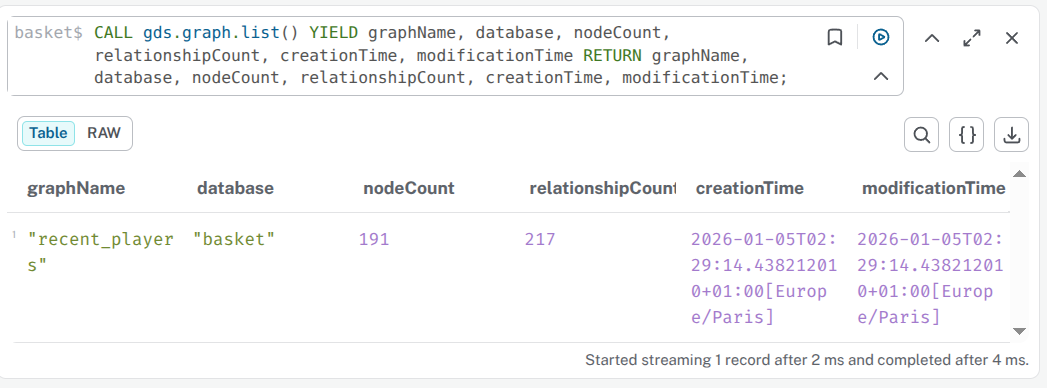
\includegraphics[width=\linewidth]{graph_list.png}
    \caption{We can see the list of projections.}
    \label{fig:projlist}
\end{figure}



\section{Analysis}

\subsection{Similarity Analysis}

A similarity function can be defined as a function that takes two input $x$ and $y$, and that ouptuts a score, generally between $0$ and $1$ (though sometimes between $-1$ and $1$) determining how close the two inputs are.

Several similarity functions are implemented in GDS.

\subsubsection{Jaccard Similarity}

This similarity functions measures overlap between sets. When applied to a graph such as ours, the sets are the respective nodes' set of neighbours. Meaning that if for two nodes we get a score of $1.0$, those two nodes have exactly the same neighbours.

We will compute the Jaccard Similarity for the top 10 nodes (in terms of degree\footnote{Number of relationships.}) of each of our projection (bipartite and monopartite).

For the bipartite graph, we get the following result. (Fig. \ref{fig:jaccard})

\begin{lstlisting}
// Top-10 Players by degree (to Teams) + Jaccard similarity (Players vs Players)
CALL {
  CALL gds.degree.stream(
    'bipartite',                               // <-- your bipartite projection name
    { nodeLabels: ['Player'], relationshipTypes: ['PLAYED_IN'] }
  )
  YIELD nodeId, score
  RETURN collect(nodeId)[0..10] AS topPlayers
}
CALL gds.nodeSimilarity.filtered.stream(
  'bipartite',
  {
    sourceNodeFilter: topPlayers,               // only compute for these 10 as sources
    targetNodeFilter: 'Player',                 // compare only against Players
    similarityMetric: 'JACCARD',
    topK: 20,                                   // best 20 matches per source player
    similarityCutoff: 0.1                       // optional
  }
)
YIELD node1, node2, similarity
RETURN
  gds.util.asNode(node1).fullGivenName AS player,
  gds.util.asNode(node2).fullGivenName AS similarPlayer,
  similarity
ORDER BY similarity DESC, player;
\end{lstlisting}
\subsection{Community detection}

\begin{figure}[htbp]
    \centering
    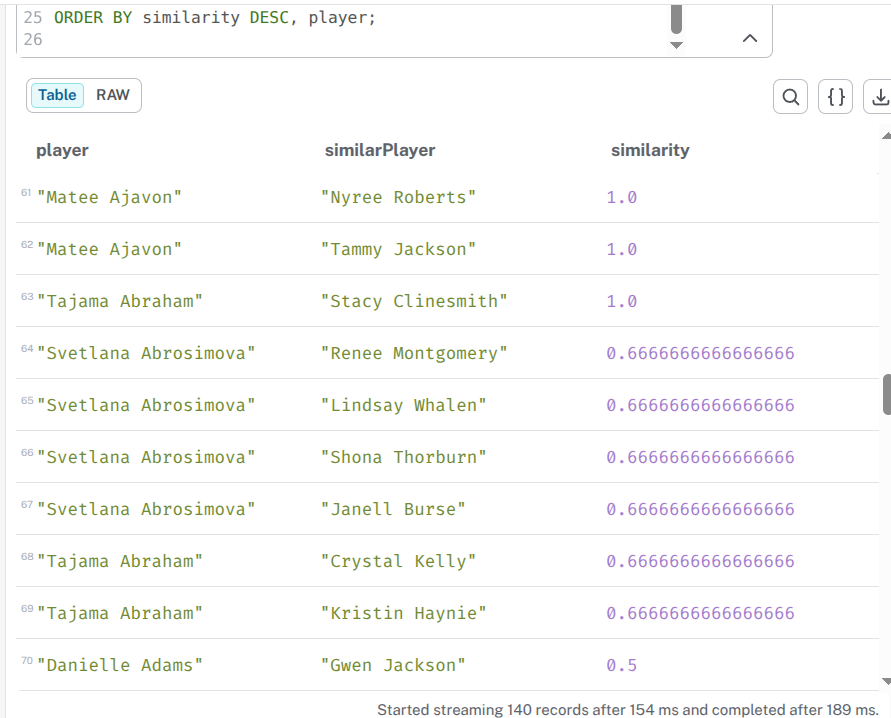
\includegraphics[width=\linewidth]{jaccard_bipartite.png}
    \caption{We compute the Jaccard on the bipartite projection.}
    \label{fig:jaccard_bi}
\end{figure}

The similarity score goes gradually from $1.0$ to $0.33$. This indicates that all of the top 10 nodes share at least one common neighbor. In addition, a lot of scores are $1.0$, meaning two players share exactly the same team history (regardless of the dates).

Now, with the monopartite graph:

\begin{lstlisting}
CALL {
  CALL gds.degree.stream(
    'monopartite',
    { nodeLabels: ['__ALL__'], relationshipTypes: ['__ALL__'] }
  )
  YIELD nodeId, score
  RETURN collect(nodeId)[0..10] AS topPlayers
}
CALL gds.nodeSimilarity.filtered.stream(
  'monopartite',
  {
    sourceNodeFilter: topPlayers,
    targetNodeFilter: '__ALL__',
    similarityMetric: 'JACCARD',
    topK: 20,
    similarityCutoff: 0.1
  }
)
YIELD node1, node2, similarity
RETURN
  gds.util.asNode(node1).fullGivenName AS player,
  gds.util.asNode(node2).fullGivenName AS similarPlayer,
  similarity
ORDER BY similarity DESC, player;
\end{lstlisting}

\begin{figure}[htbp]
    \centering
    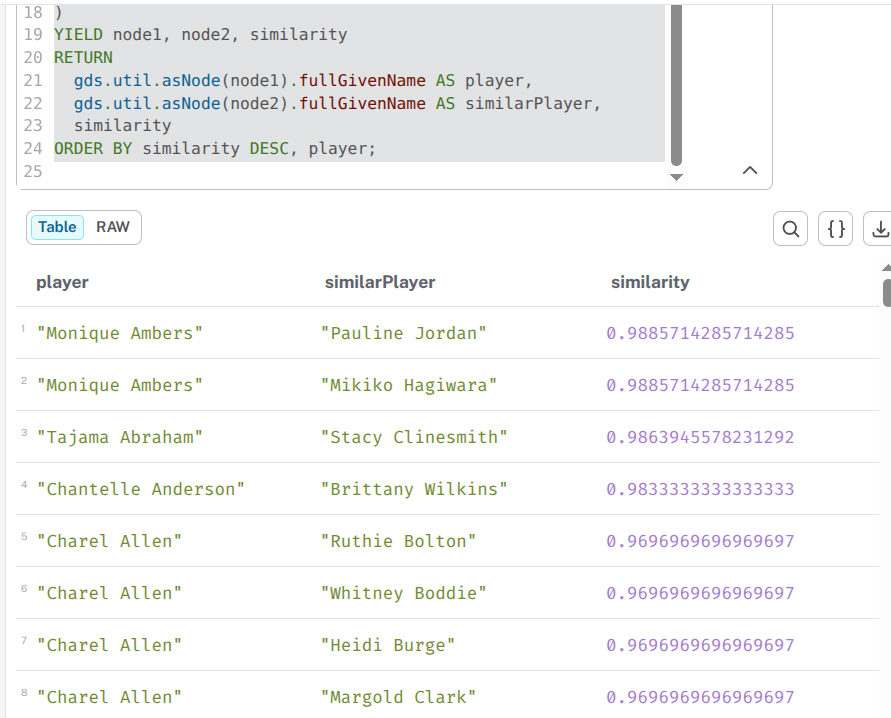
\includegraphics[width=\linewidth]{jaccard_monopartite.png}
    \caption{We compute the Jaccard on the monopartite projection.}
    \label{fig:jaccard_monopartite}
\end{figure}

The results we get (Fig \ref{fig:jaccard_monopartite}) provide us with a good visualisation of players sharing a common history. For example, at the very top, we have Monique Ambers and Pauline Jordan, who both did their careers in the Phoenix Mercury and the Sacramento Monarchs.

\subsection{Community Analysis}

A community can be loosely defined as a group of nodes that are more strongly connected to each other than to the rest of the graph.

This allows us to detect communities, meaning group of nodes forming groups within the graph.

One such algorithm is Louvain. Louvain is an algorithm meant for monopartite graphs only. As such, we will only run it on our \verb|monopartite| projection.

\subsubsection{Louvain}

\begin{lstlisting}
CALL gds.louvain.write(
  'monopartite',
  {
    writeProperty: 'communityId'
  }
)
YIELD communityCount, modularity, ranLevels, nodePropertiesWritten;
\end{lstlisting}

Notice this part \verb|WHERE 'Player' IN labels(n)|, whic filters out non-Player nodes.

\begin{figure}[htbp]
    \centering
    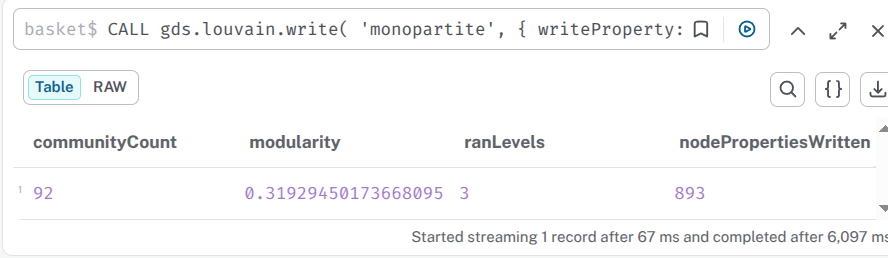
\includegraphics[width=\linewidth]{louvain_monopartite.png}
    \caption{Detecting communities}
    \label{fig:louvain_monopartite}
\end{figure}

As we can see in figure \ref{fig:louvain_monopartite}, Louvain identified 92 communities. They reveal what teams the players played in, as this is based on the graph's relationships (which in our mono-partite projection only reveals the teams the players played in).

\begin{figure}[htbp]
    \centering
    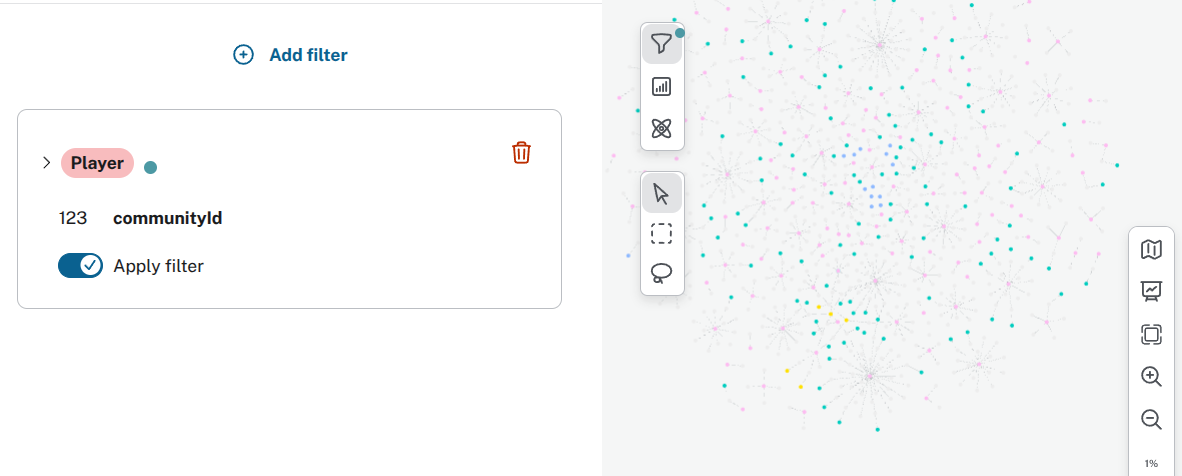
\includegraphics[width=\linewidth]{louvain_monopartite_filter.png}
    \caption{Detecting communities}
    \label{fig:louvain_monopartite_filter}
\end{figure}

As we can see in Fig. \ref{fig:louvain_monopartite_filter}, we can then filter the view by community ID. (Community IDs go above 92 because they are not sequential.)

Future work may include creating new relationships between Players (for instance, if they went to the same high school or college), and run Louvain specifically on these relationships or on all relationships together, to see the impact it has on communities. However, Louvain is not deterministic. Change will happen every time it is run.

\subsubsection{Connected Components}

Connected Components is an algorithm useful for detecting independent communities in a graph. It is also an algorithm we can run on our bipartite graph.

\begin{lstlisting}
CALL gds.wcc.stream('bipartiteProj')
YIELD nodeId, componentId
RETURN gds.util.asNode(nodeId).fullGivenName AS Player,
       componentId
ORDER BY componentId
\end{lstlisting}

The vast majority of the returned Players belong to "componentId" number 0. Others however belong to a separate "componentId" in which they are the only Player.

What this means is that most players belong to the same component (it is possible to access any player from any other player by following a stream of relationships). Some others however are completely isolated, because they are not linked to any other player. (Figure \ref{fig:connected}.)

\begin{figure}[htbp]
    \centering
    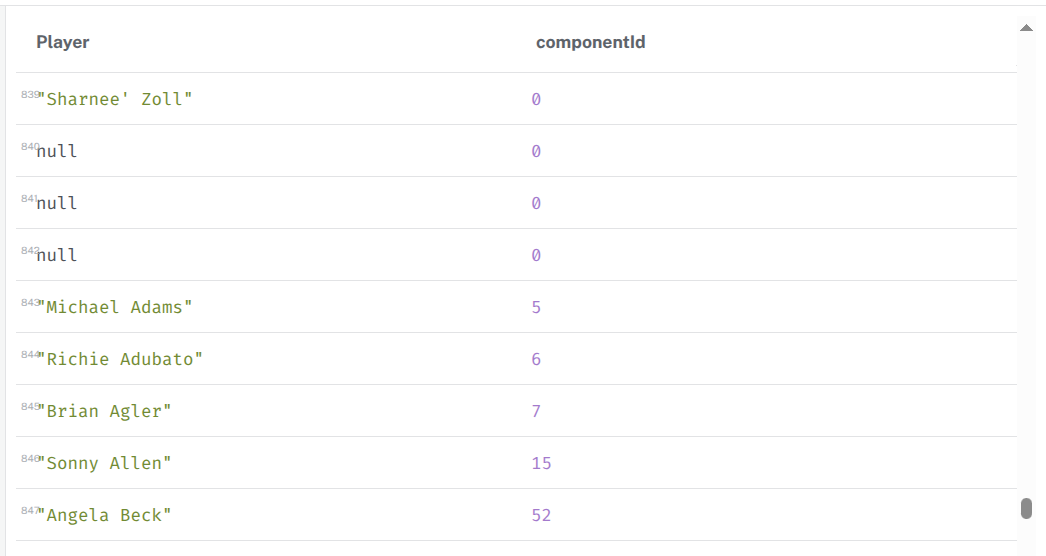
\includegraphics[width=\linewidth]{components.png}
    \caption{Most nodes are connected together, apart from a few isolated ones.}
    \label{fig:connected}
\end{figure}



\end{document}